% Lezione 2/2024-02-28
% - Introduzione alla descrizione quantitativa del moto (cinematica?)
% - cinematica del punto materiale da una a piu' dimensioni: moto rettilineo uniforme, piano cartesiano
% - equazioni del moto, con notazione vettoriale
% Esercitarsi su: moto rettilineo uniforme, vettori e trigonometria, sistemi di riferimento cartesiani e algebra sul piano cartesiano


\chptr{Descrizione del moto}

\section{Introduzione al moto del punto materiale}
Un corpo è in moto quando la sua posizione cambia nel tempo. Nel descrivere il
moto, si introdurrà la seguente semplificazione: gli oggetti in moto saranno
trattati come \textit{punti materiali}, ovvero concentrati in un punto
adimensionale. Il modello del punto materiale è un buon punto di partenza per
comprendere bene il fenomeno del moto (cominciare dal quadro attuale, ovvero
quello della relatività ristretta, sarebbe interessante ma ostico). In particolare,
\textit{le dimensioni dell'oggetto del quale si intende studiare il moto saranno
considerate trascurabili rispetto a quelle dell'ambiente circostante}.

\subsection{Sistemi di riferimento}
Abbiamo detto che il moto è caratterizzato da un cambiamento di posizione. Il primo
passo nella descrizione del moto di un corpo consiste quindi nello stabilire il
modello da adottare per catturare il concetto di \textbf{posizione}. Sappiamo già
che i modelli della fisica si basano sul linguaggio matematico; il modello più
naturale che si possa adottare è dunque un sistema di assi cartesiani. Da qui, la
posizione del corpo può essere specificata mediante coordinate. Una speciale
coordinata è il tempo.

La scelta del sistema di riferimento di assi cartesiani è del tutto arbitraria,
ma una volta fissata è necessario essere coerenti con essa.


\section{Moto rettilineo uniforme}

\begin{marginfigure}
    \centering
    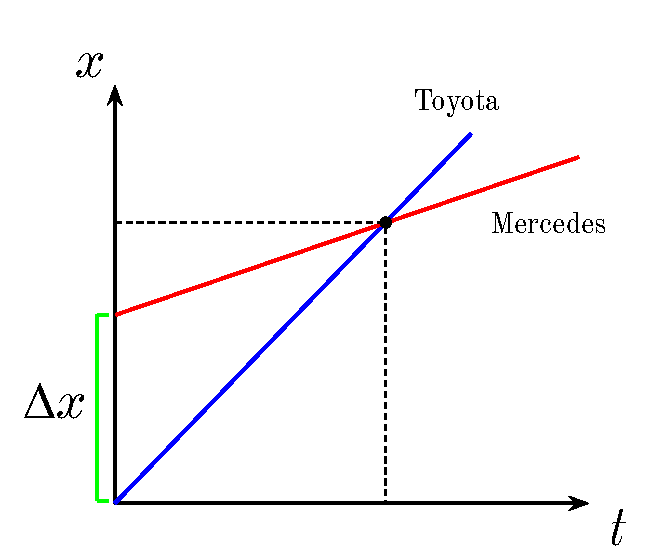
\includegraphics[width = \marginparwidth]{figures/sorpasso.pdf}
    \caption{Un caso di sorpasso}
\end{marginfigure}

\[  \]
\[ x(t) = x_i + v(t - t_i)  \]